\subsection{Geometry and material properties}
\label{sub:geometry_and_material_properties}

At first the FEM model was created considering a safety factor of $2$ and a maximum operating frequency range of $0-8 [Hz]$.

From theory, we know that in a FEM model the geometry and in particular the length of the elements is determinant when it comes to the accuracy of the results, given that a too coarse mesh can lead to inaccurate results, while a too fine mesh can lead to a high computational cost.
Because of this, the maximum length of the single elements was determined as:

\begin{equation}
    L_{\text{max}} = \sqrt{\frac{\pi^2}{\eta \Omega_{max}} \sqrt{\left(\frac{EJ}{m}\right)_{min}}} \approx 12 \quad [m]
\end{equation}

Once the model has been discretized and the geometrical and material properties have been assigned to each element based on the suggested values reported in Table \ref{tab:parameters}, the model was imported in adequate \texttt{MATLAB} data structures.

The output of this first step is a schematized version of the harbour crane, as shown in Figure \ref{fig:harbour-crane-scheme}.

\begin{figure}[H]
    \centering
    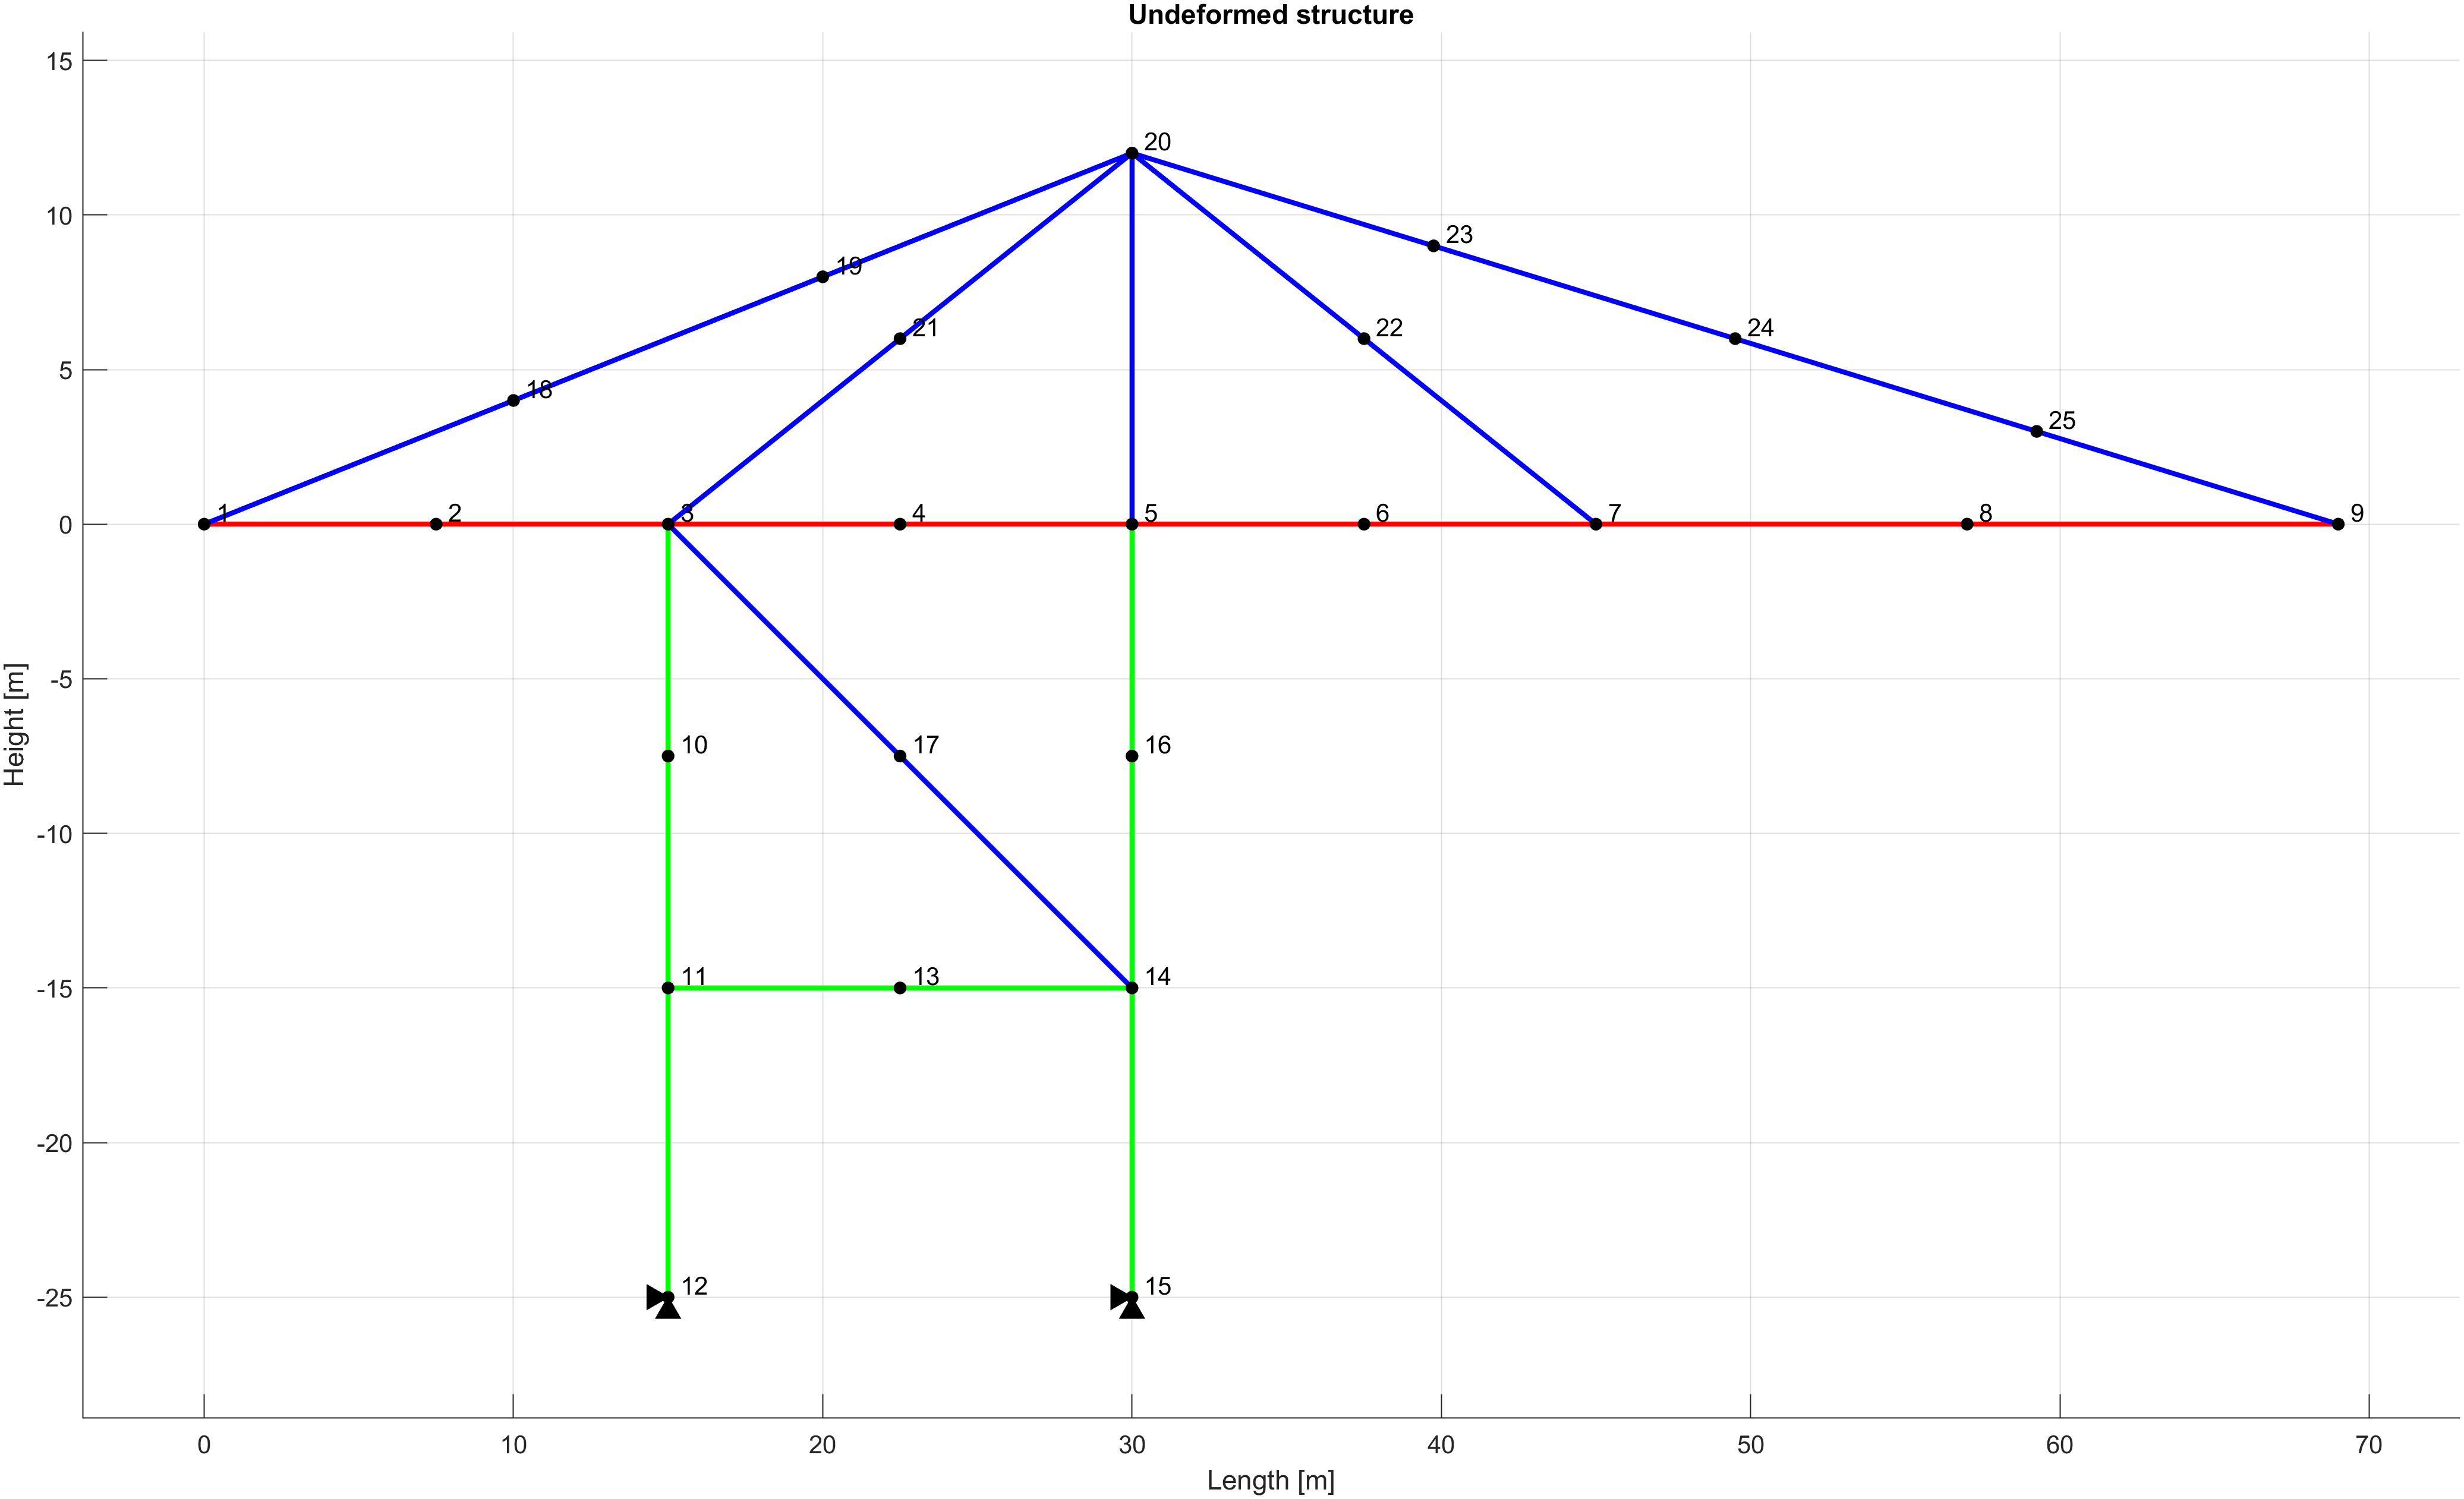
\includegraphics[width=0.7\textwidth]{img/MATLAB/undeformed-structure.png}
    \caption{Harbour crane scheme. Node naming: [\textbf{A}, \textbf{B}, \textbf{C}, \textbf{D}, \textbf{O2}] = [\textbf{\#9}, \textbf{\#14}, \textbf{\#1}, \textbf{\#7}, \textbf{\#15}]}
    \label{fig:harbour-crane-scheme}
\end{figure}

As suggested/requested by the assignment, the harbour crane was modelled as a 2D frame structure composed of beam elements.
As an assumption, the joints \textbf{A} and \textbf{C} were assumed to be rigid connections, even if in reality those elements are usually not capable of transmit bending moments, but only axial forces (hinge connections type).
This assumption was made to simplify the model and the analysis.
However, the model could be easily modified to include the possibility of free relative rotations in those joints by adding another degree of freedom to the system.

With respect to the schematic representation of the crane of Figure \ref{fig:harbour-crane-scheme}, the parameters of the structure are provided in Table \ref{tab:parameters}.

\begin{table}[H]
    \centering
    \begin{tabular}{|r|c|c|c|}
        \hline
        ~           & \textbf{m [kg/m]} & \textbf{EA [N]} & \textbf{EJ [Nm$^2$]} \\
        \hline
        Red beams   & $312$             & $8.2E9$         & $1.4E9$              \\
        Green beams & $200$             & $5.4E9$         & $4.5E8$              \\
        Blue beams  & $90$              & $2.4E9$         & $2.0E8$              \\
        \hline
    \end{tabular}
    \caption{Parameters of the structure}
    \label{tab:parameters}
\end{table}

For the rest of the analysis, we will assume a proportional damping matrix $[C] = \alpha [M] + \beta [K]$ with $\alpha = 0.01 [\frac{1}{s}]$ and $\beta = 2E-4 [s]$